\documentclass[12pt]{article}
\usepackage[utf8]{inputenc}
\usepackage[margin=1in]{geometry}
\usepackage{amsmath}
\usepackage{graphicx}
\graphicspath{ {./images/} }

\author{Neelu Saraswatibhatla (srns2)}
\title{MLRD Supervision 3}
\date{\vspace{-5ex}}

\begin{document}

\maketitle

\section*{Markov assumption}

The first-order Markov assumption is that the state at time $t$ depends only on the state at time $t-1$, i.e. $P(X_t | X_{t-1}, X_{t-2}, \ldots, X_1) \approx P(X_t | X_{t-1})$, where $X_t$ is the state at time $t$.
This means that we don't need to keep lists of state probabilities at loads of different timesteps and calculate probabilities depending on states at many different timesteps, we just calculate probabilities based on the states at the previous timestep.
This is known as the Limited Horizon as we can only "see" back 1 step, so we only have a "horizon" of 1 timestep.

The other assumption HMMs use is that of output independence. This is the assumption that the probability of the current output only depends on the current state, and on no previous or future states or outputs, i.e. $P(O_t | X_1, \ldots, X_t, \ldots, X_T, O_1, \ldots, O_t, \ldots, O_T) \approx P(O_t | X_t)$, where $X_t$ and $O_t$ are the state and observation respectively at time $t$, and $T$ is the final timestep in the Markov chain.
This means that we only need to look at the probabilities of states at the current timestep to determine emission probabilities, and don't need to look forward or back and previous or future states or observations.

\section*{HMM Artificial data}
\begin{enumerate}
    \item You need the list of states, list of observations, and the transition and emission probability matrices.
    \item Start at the start state. Then, generate the Markov chain. This can be done by using the transition matrix, starting at the start state and randomly selecting a next state with the probability distribution provided by the transition matrix, and then continuing until the end state has been reacher.

    Then, the observations can be generated in a similar way by going through the Markov chain (except the start and end states) and randomly selecting an observation for each state according to the distributions stipulated by the emission matrix.
    
    \item This can occur when there are multiple end states rather than just one. For example, in the weather example with a start state and hidden states Raining and Not Raining, there could be two end states: ``There is flooding" and ``There is no flooding" by the end of the month.
\end{enumerate}

\section*{Smoothing in HMMs}
\begin{enumerate}
    \item Add-one smoothing helps improve accuracy by preventing one probability in a product of probabilities being 0 from making the overall product 0, ignoring all the other probabilities in the product. However this means that the probability is made slightly less accurate. If we are sure that none of the constituent probabilities of a product will be 0 then there is no point in using add-one smoothing and it can be counterproductive.
    \item The transition probabilites are the better candidate for smoothing. This is because some transitions will be 0 as proteins with amino acids inside the cell need to go through the membrane before they can go outside and vice versa, so the state transition probability straight from inside to outside or outside to inside is 0. Therefore we may want to smooth the transition probabilities so a transition probability of 0 doesn't make an entire product of probabilities 0.
\end{enumerate}

\section*{Viterbi and Forward algorithm}
\begin{enumerate}
    \item The formula is as follows:
    \begin{align*}
        \alpha_t(j) = \sum \limits_{i=1}^{N} \alpha_{t-1}(i)a_{ij}b_j(o_t)
    \end{align*}
    The probability of state $j$ at time $t$ ($\alpha_t(j)$) is the sum over every state $i$ of state $i$ being the state at the previous timestep ($t-1$) multiplied by the transition probability from state $i$ to $j$, multiplied by the probability of observation $o_t$ given state $j$. This is because the probability of a state depends on the previous state, as well as the transition from that previous state to the current state, and the observation at the current time.
    \item We sum over the paths as the current state depends on the previous state, so we sum over every possible previous state getting its contribution to the probability.
\end{enumerate}

\section*{Parts of Speech tagging with HMM}
\begin{enumerate}
    \item In $X_a$, the order is personal pronoun $\rightarrow$ auxiliary verb $\rightarrow$ verb, so `can' is an auxiliary verb and `fish' is a verb, so this sentence can be interpreted as ``We are able to fish".
    In $X_b$ the order is personal pronoun $\rightarrow$ verb $\rightarrow$ noun, so `can' is a normal verb and not an auxiliary verb, and `fish' is a noun, so this sentence means ``We put fish in cans".
    \item $P(X_a) = a_{03} \times a_{34} \times a_{41} \times a_{1f} = 0.60 \times 0.40 \times 0.74 \times 0.15 = 0.02664$\\
    $P(X_b) = a_{03} \times a_{31} \times a_{12} \times a_{1f} = 0.03024$\\
    $P(X_a, O) = P(X_a) \times b_3(\text{we}) \times b_4(\text{can}) \times b_1(\text{fish}) = 0.02371$\\
    $P(X_b, O) = P(X_b) \times b_3(\text{we}) \times b_1(\text{can}) \times b_2(\text{fish}) = 0.00226$\\
    \\
    The HMM takes both transition and emission probabilities into account, so it uses $P(X_a, O)$ and $P(X_b, O)$.
    \item We calculate $\delta_j(t)$ for each state $j$ for time $t = 1$, and use the helper variable $\Psi_j(t)$ to keep track of the previous state.\\
    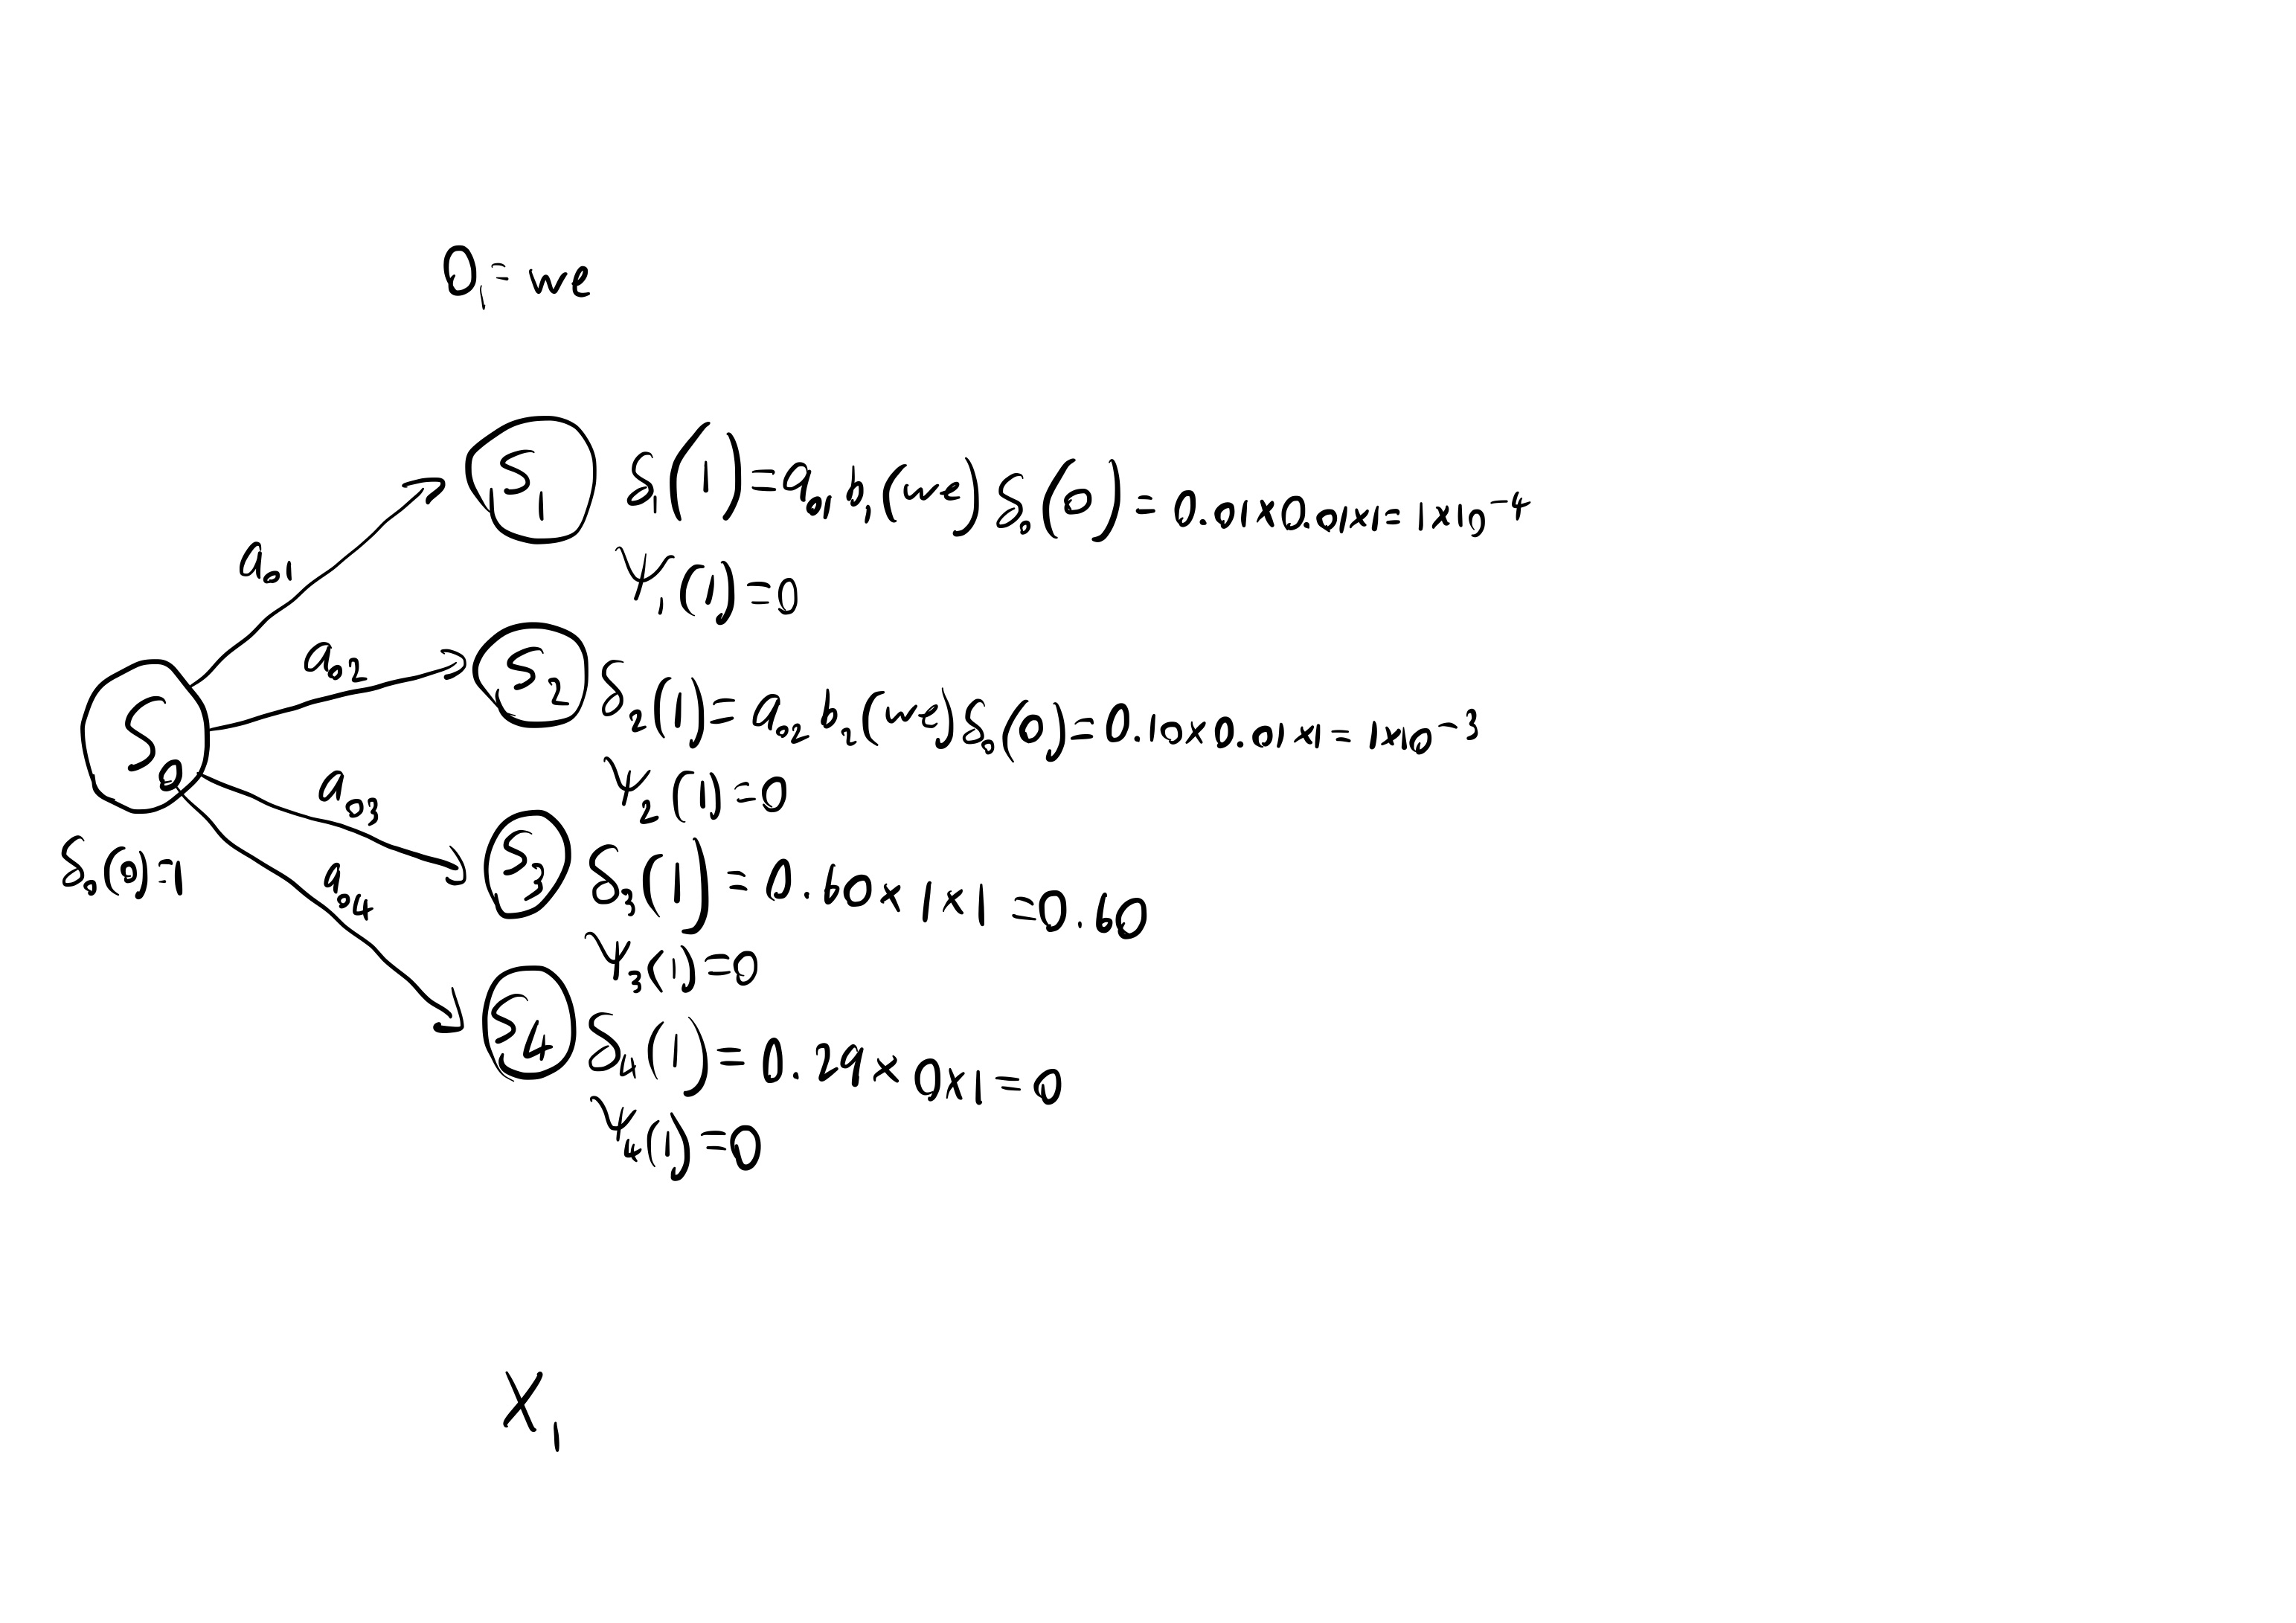
\includegraphics[scale=0.125]{3-1.jpg}\\
    We then do this again for timestep $t = 2$, but we calculate $\delta$ recursively for each state transition, i.e. each pair of states, take the maximum, and store the previous state giving us this maximum in $\Psi$.\\
    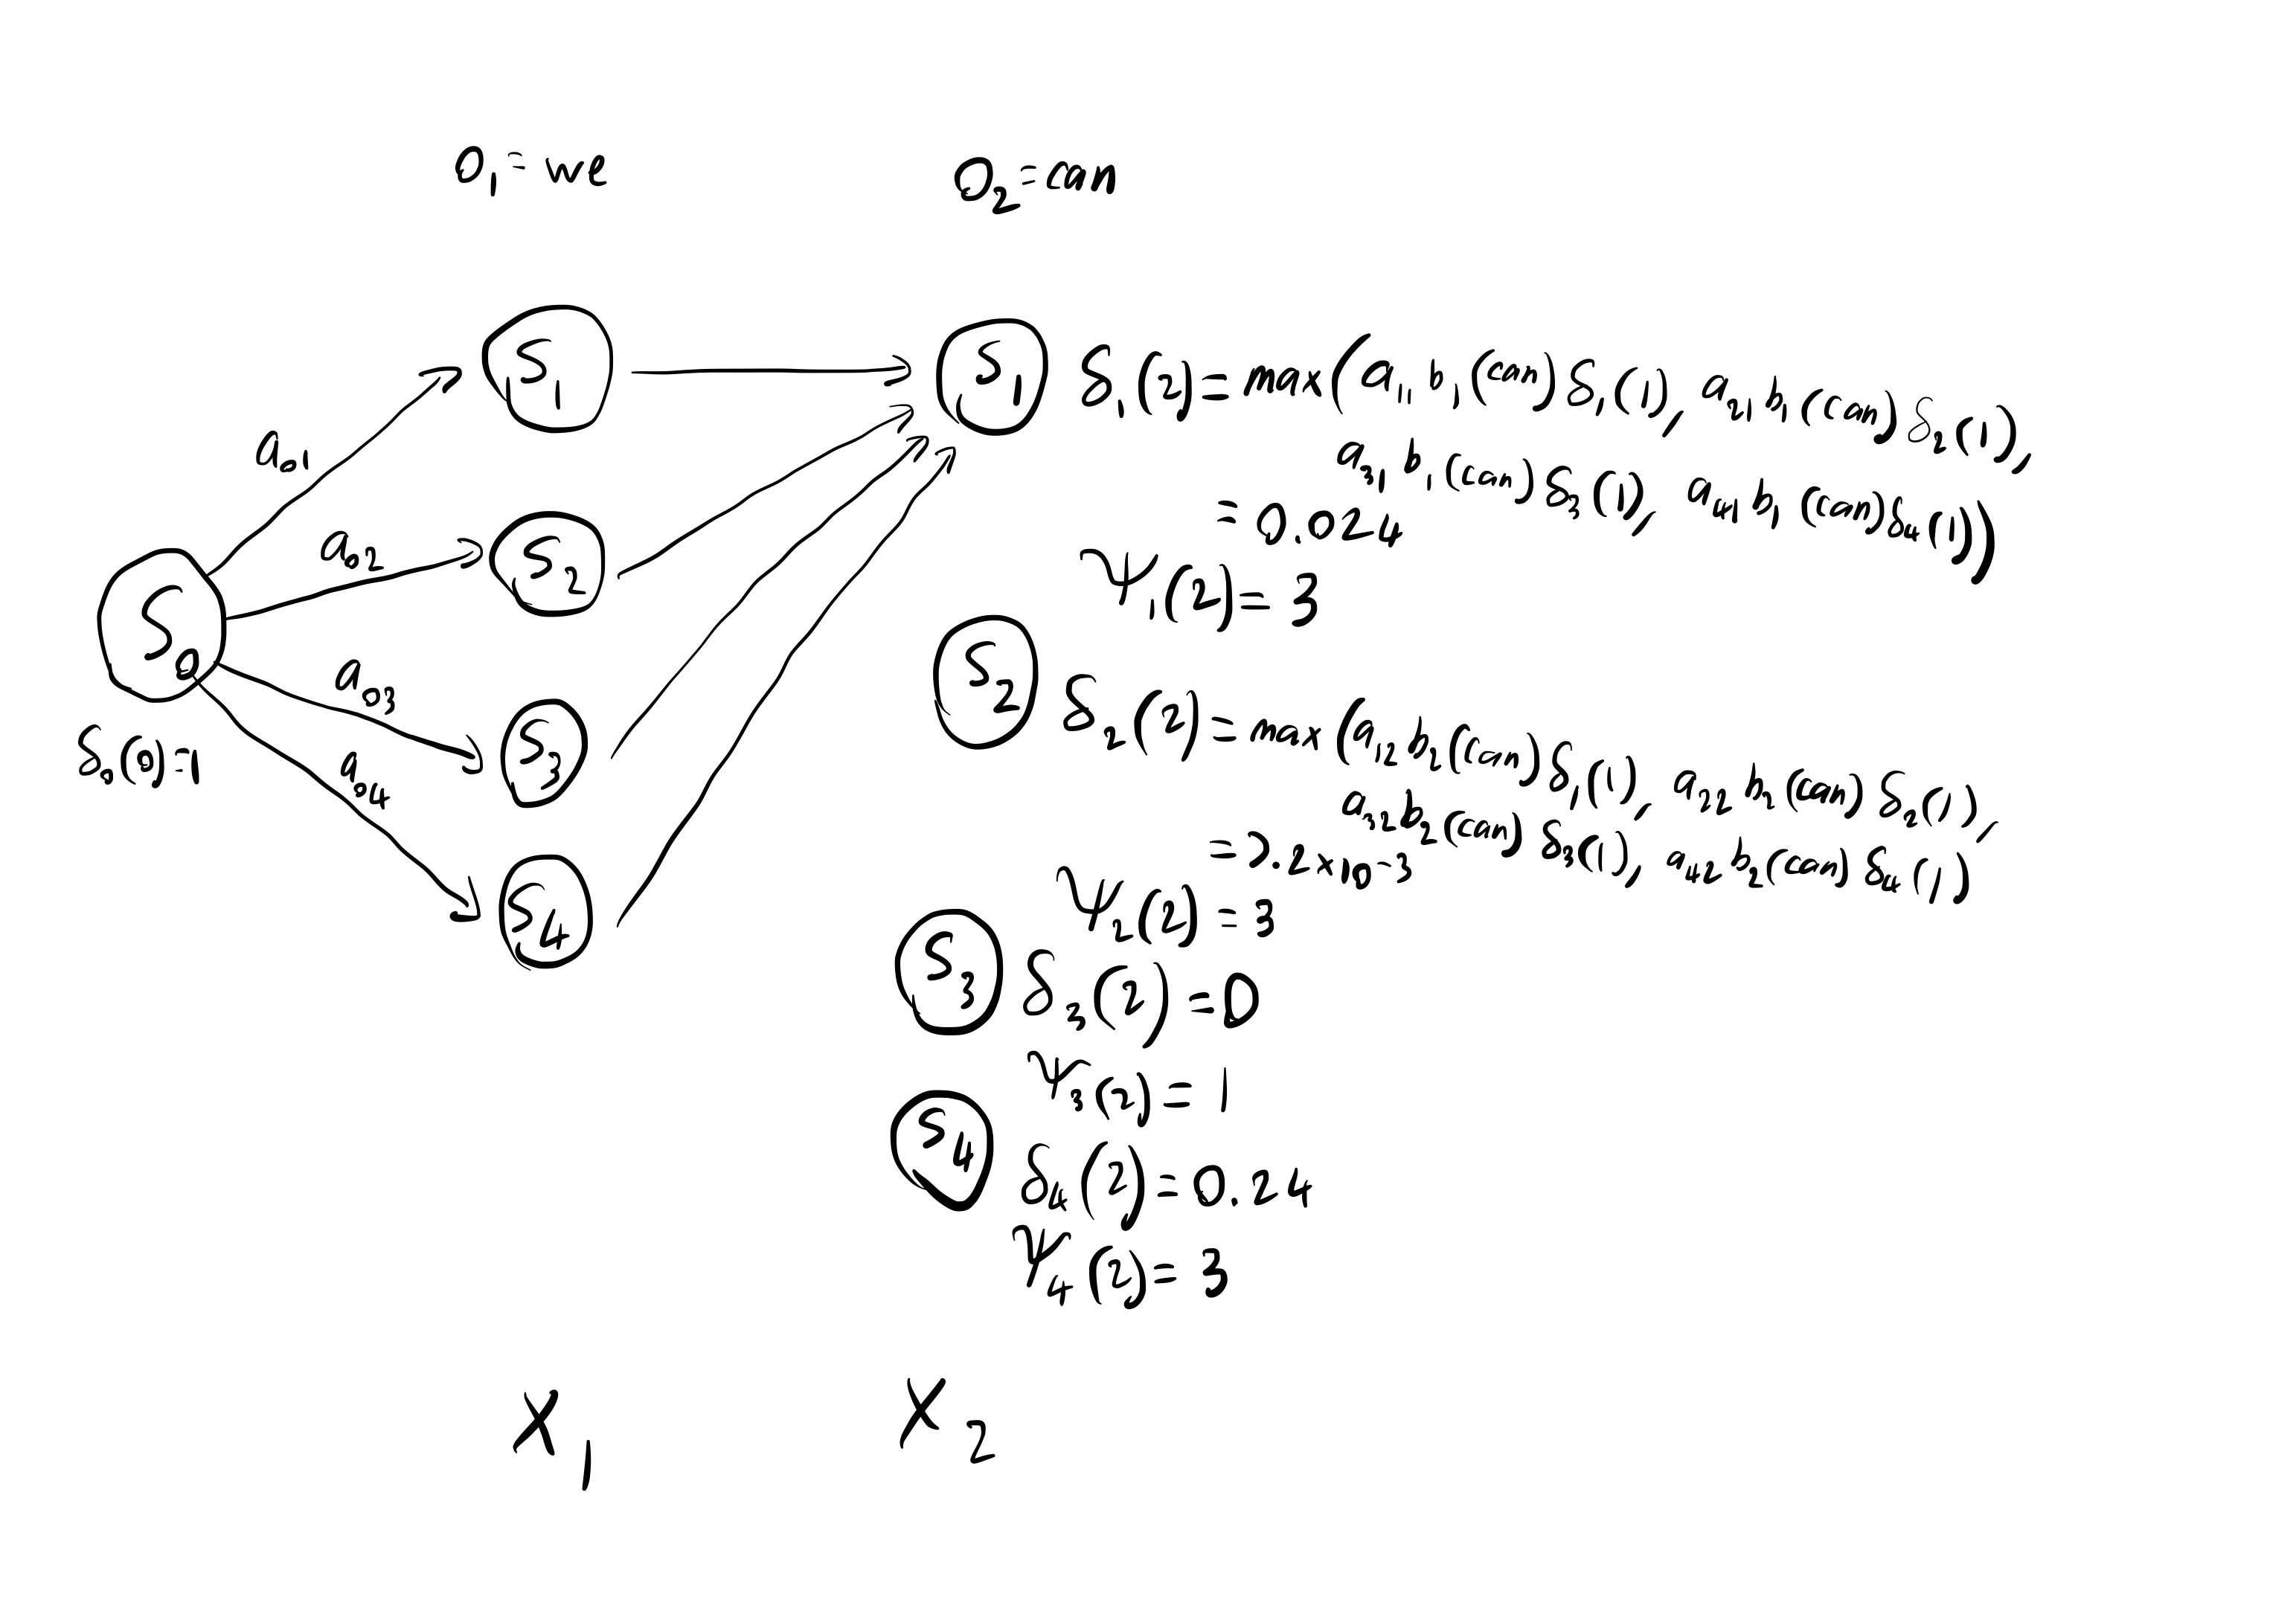
\includegraphics[scale=0.125]{3-2.jpg}\\
    This is done again for timestep $t=3$.\\
    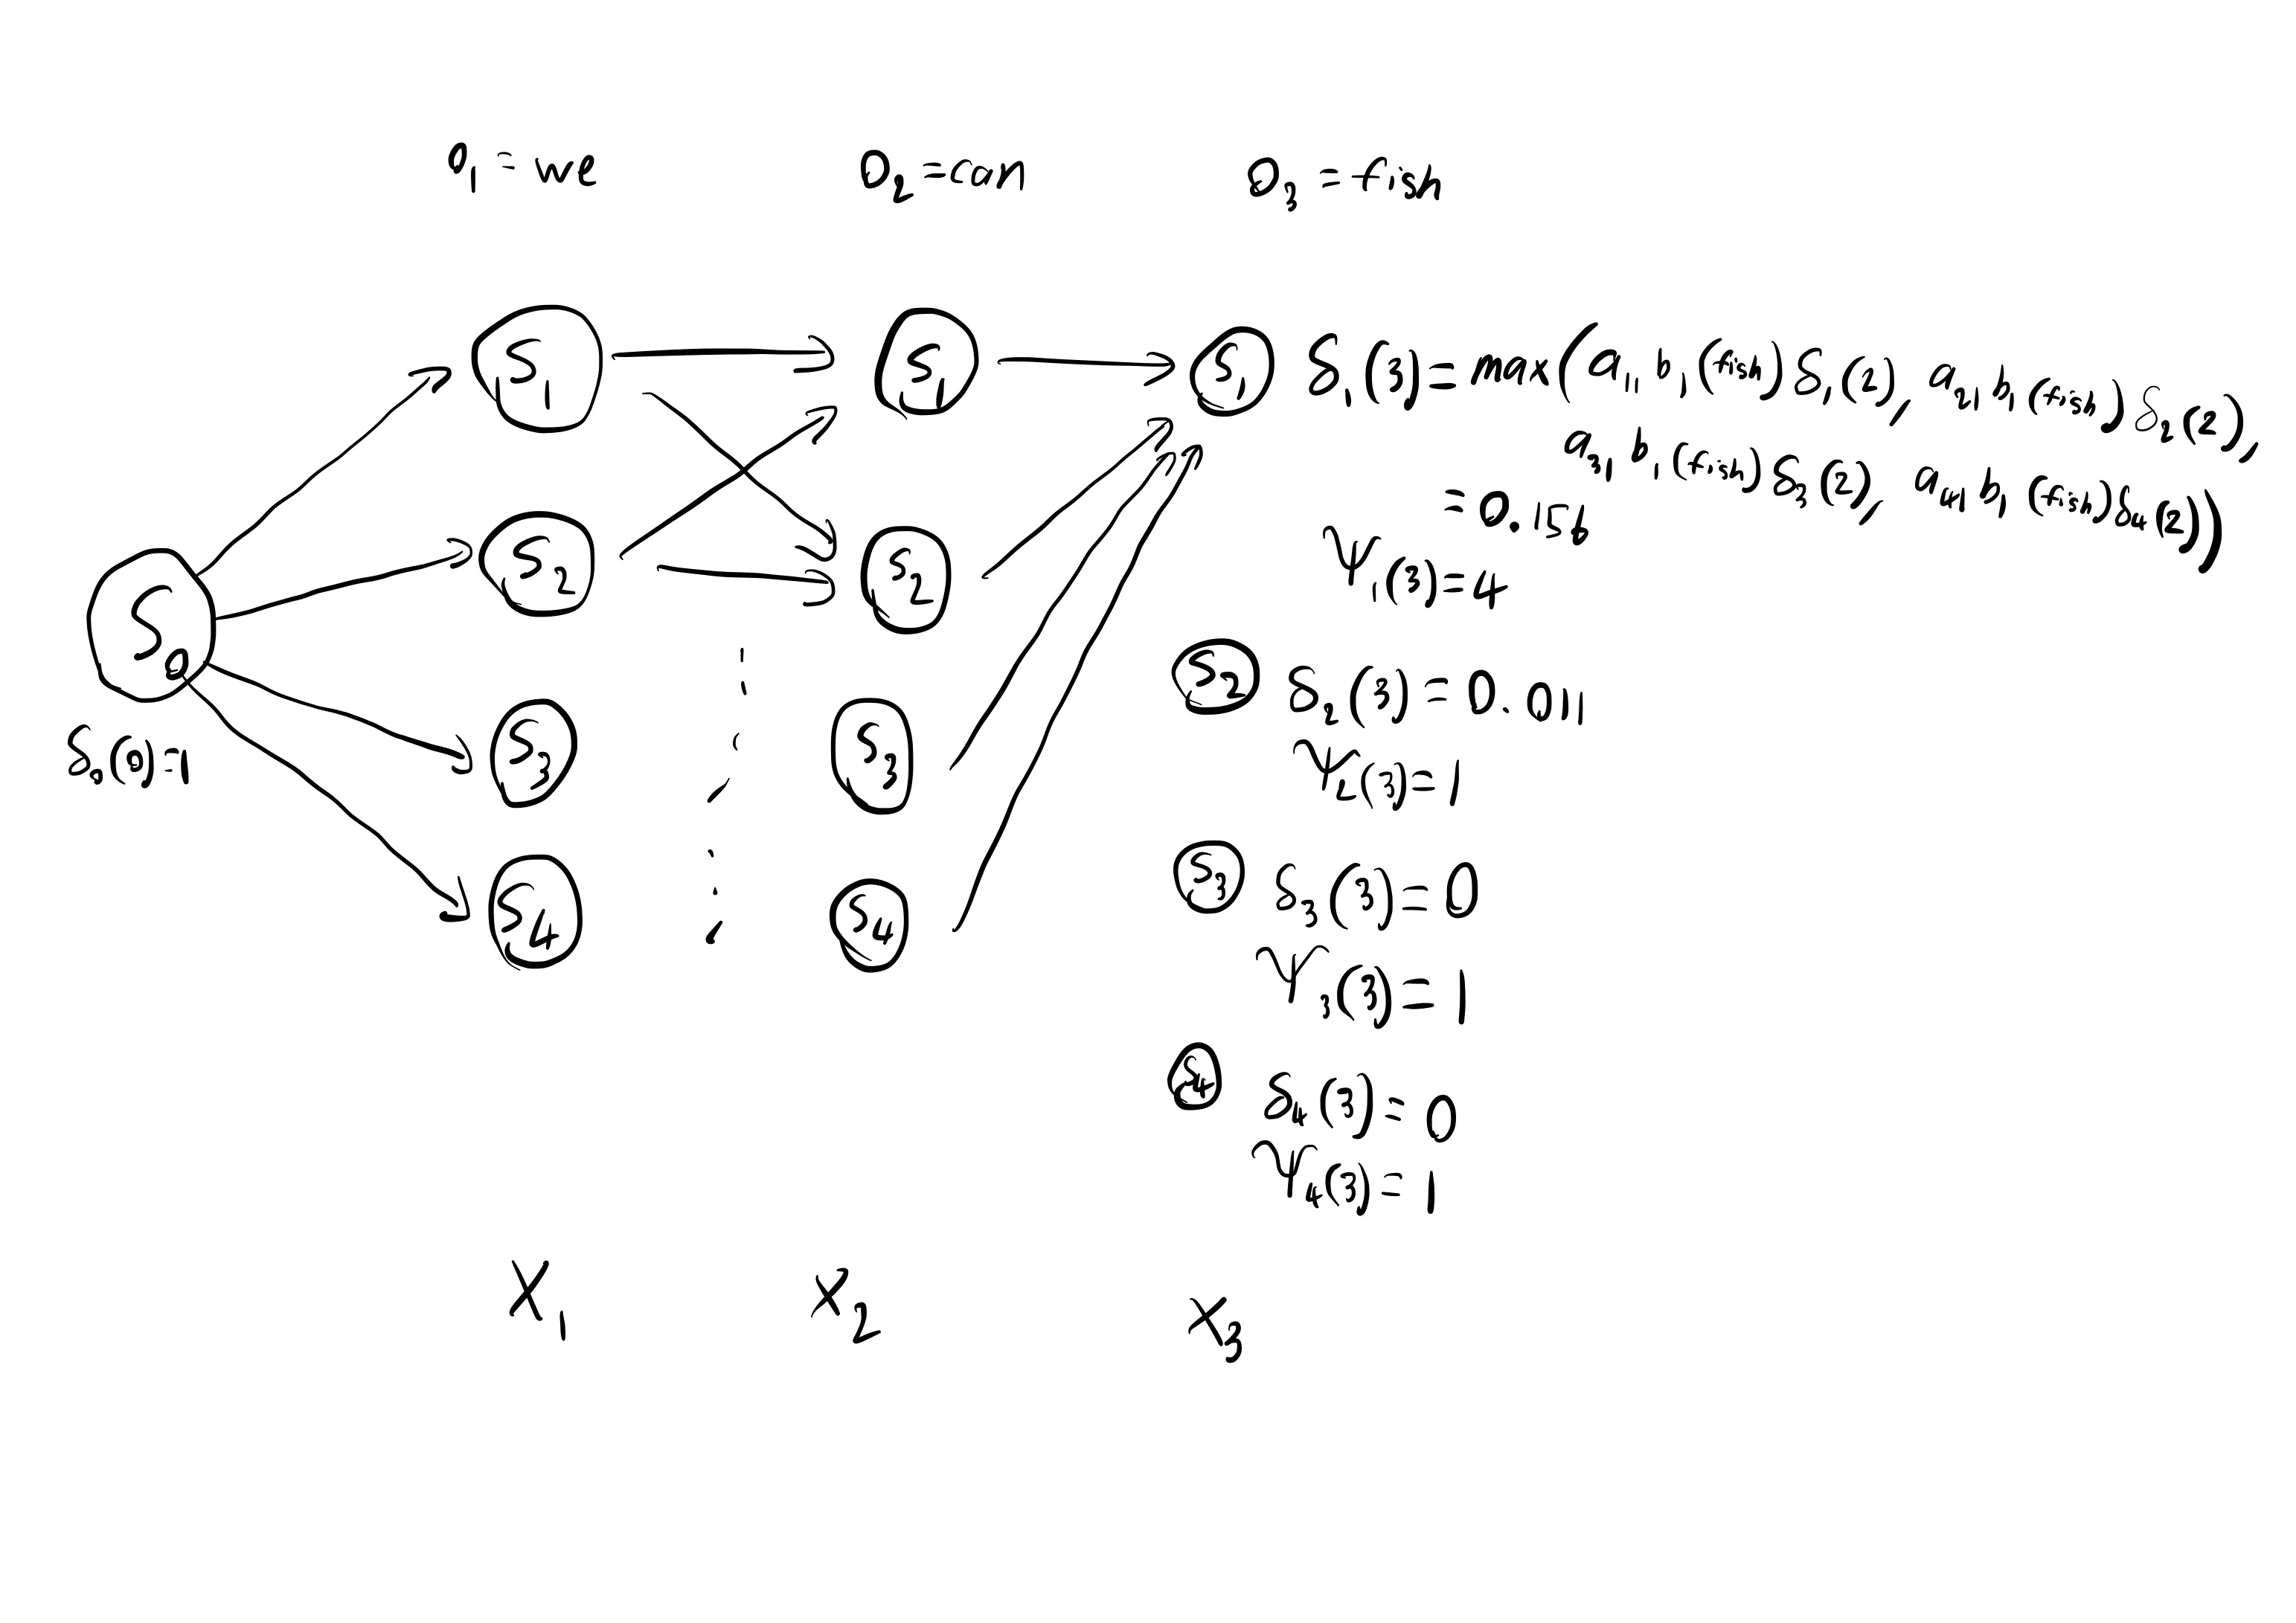
\includegraphics[scale=0.125]{3-3.jpg}\\
    We then do this for the transitions to the final state.\\
    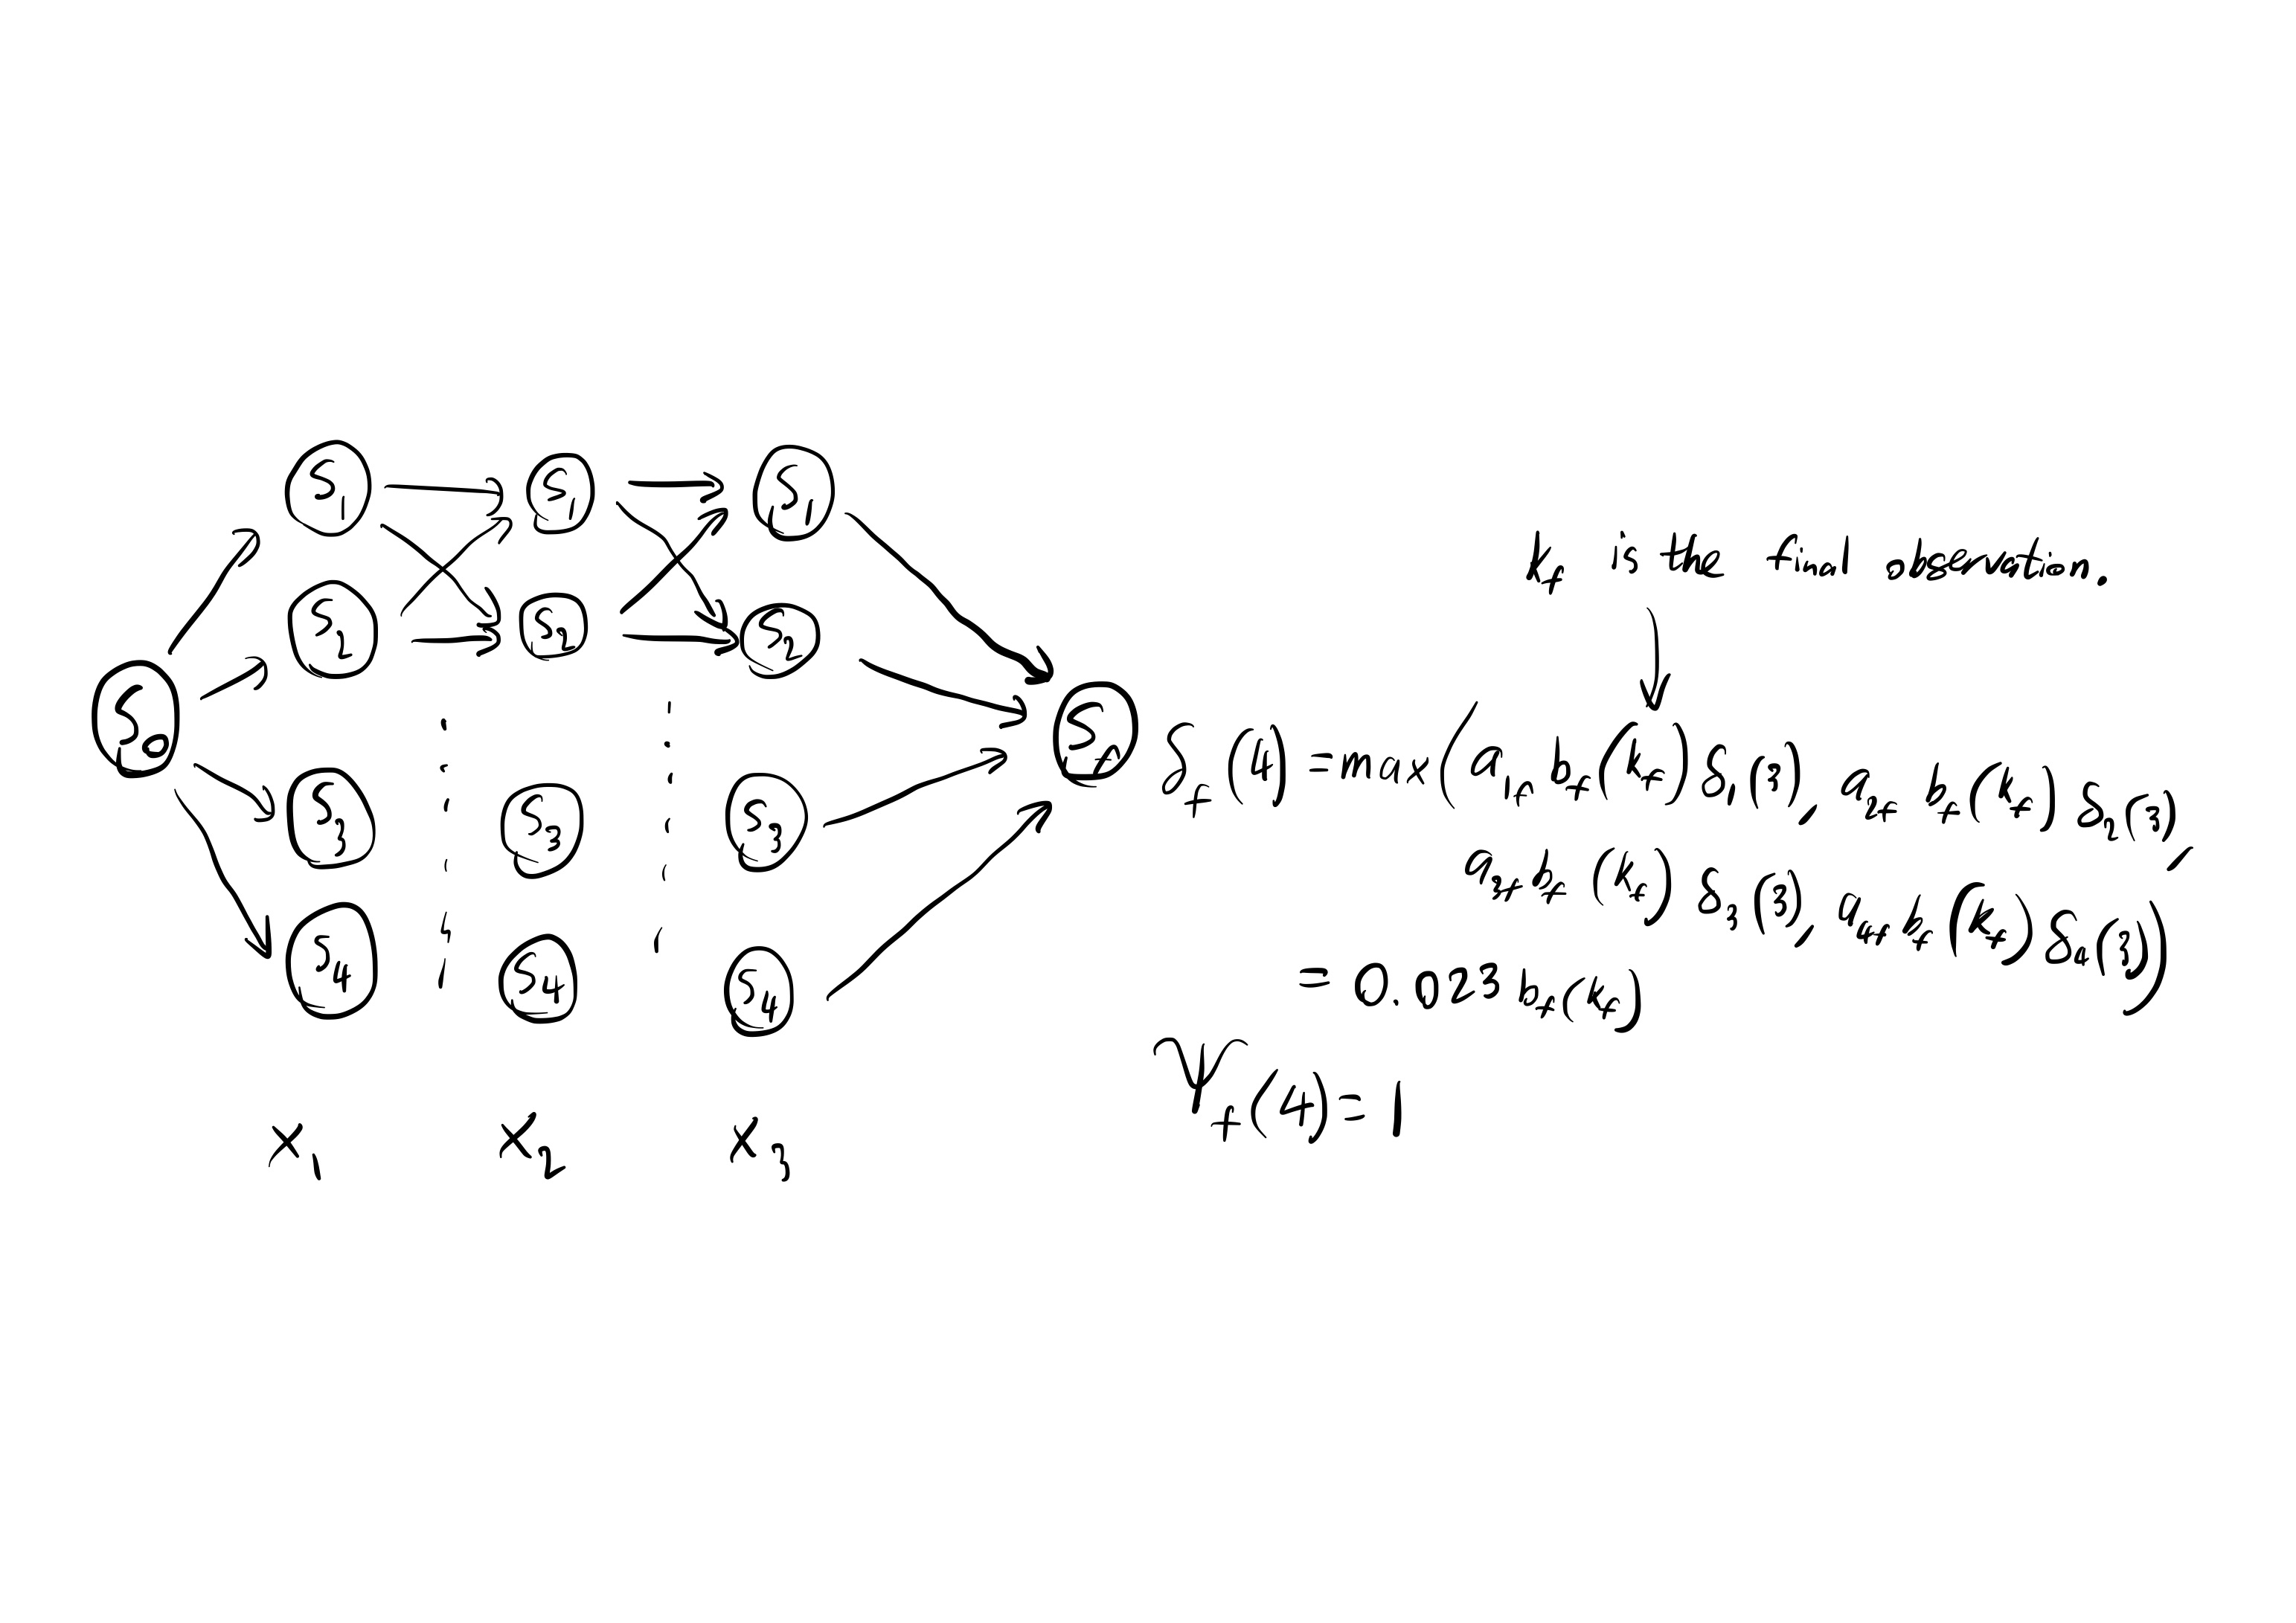
\includegraphics[scale=0.125]{3-4.jpg}\\
    We then backtrace:\\
    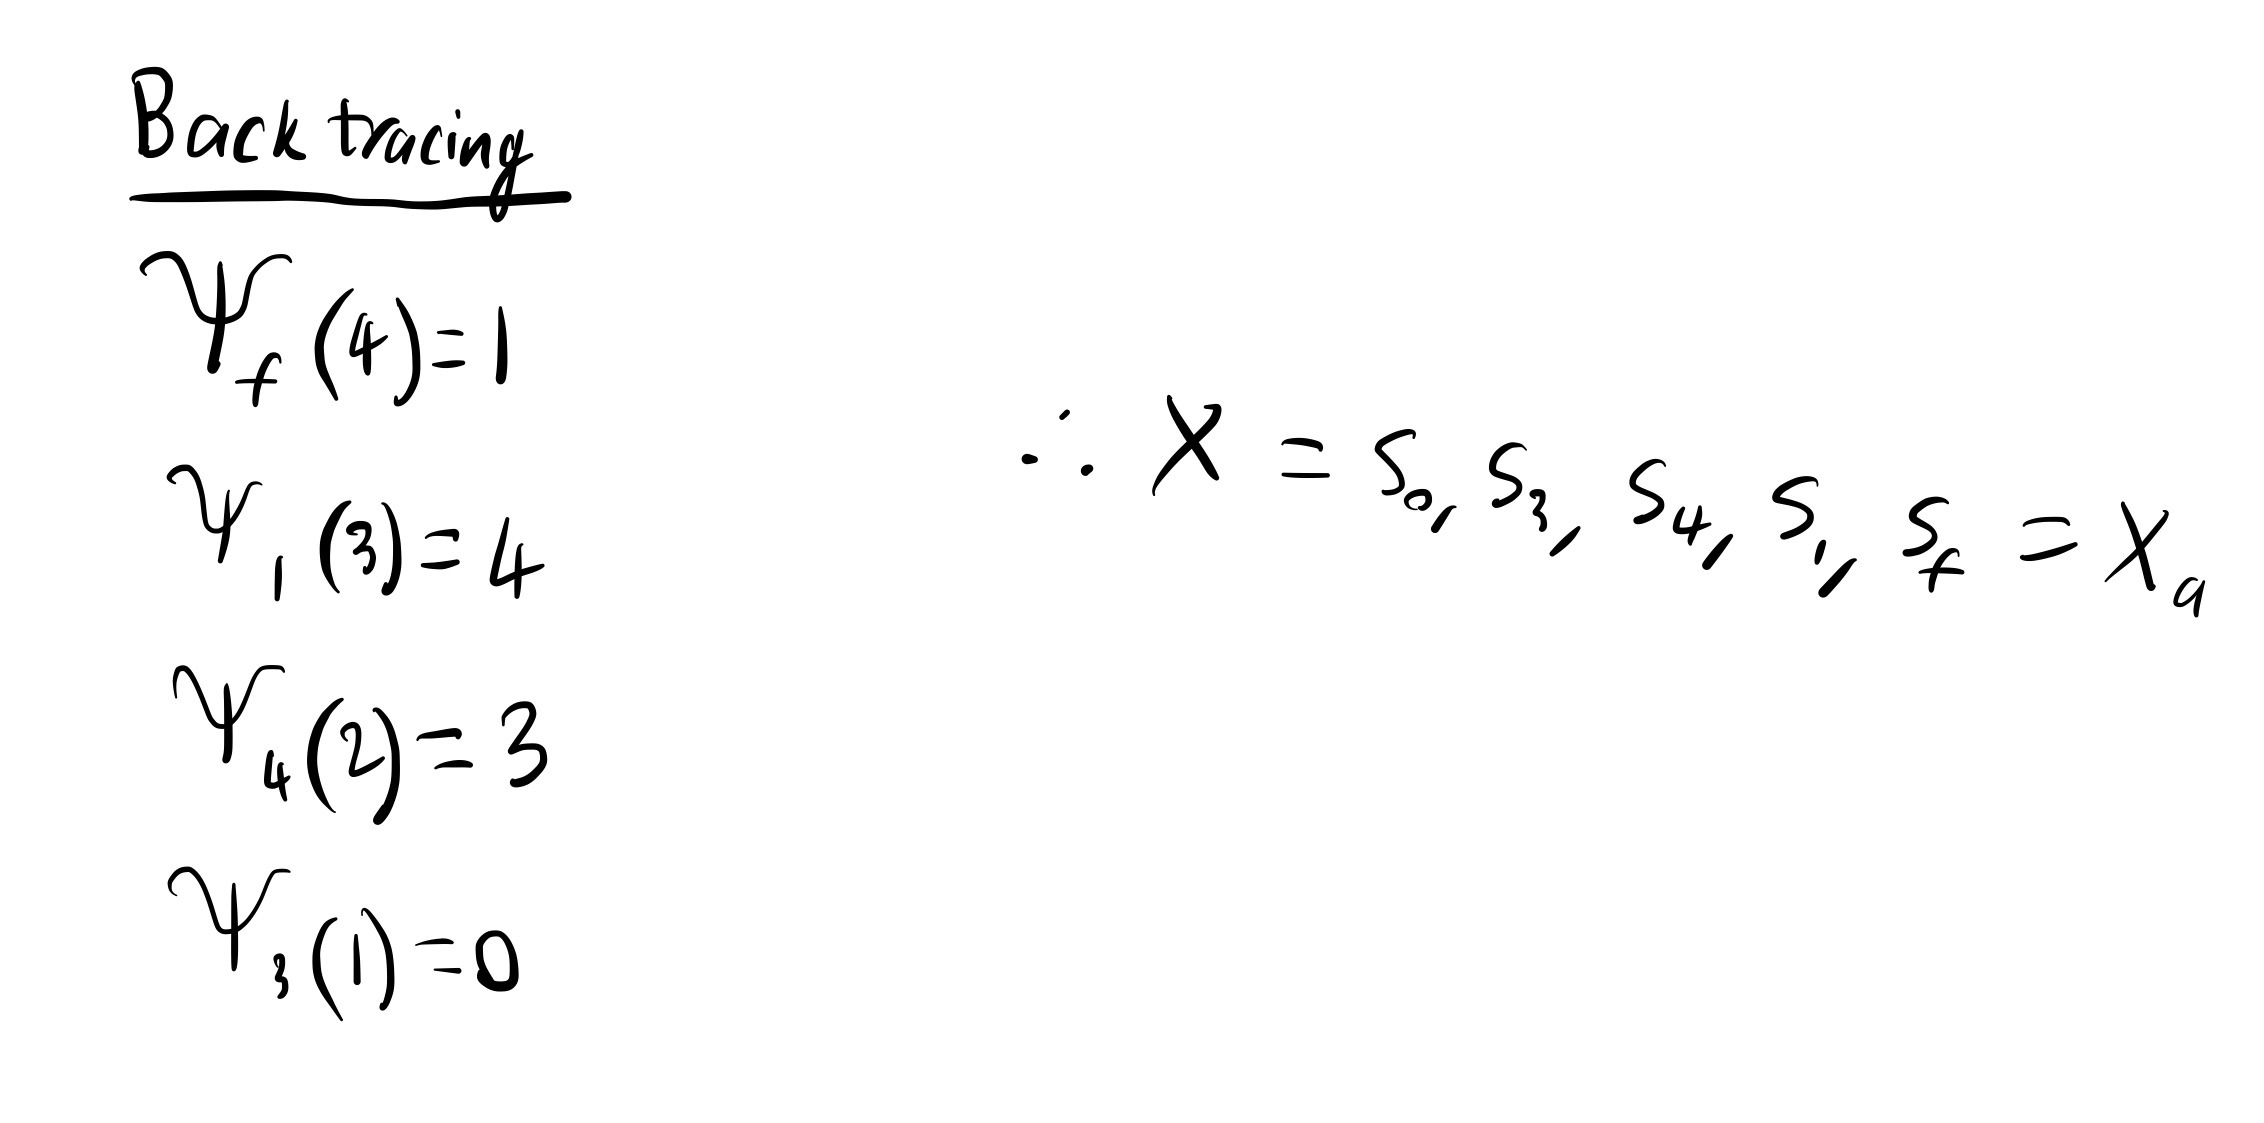
\includegraphics[scale=0.1]{3-5.jpg}\\
    We therefore get the most likely outcome to be $X_a$, i.e. $s_0, s_3, s_4, s_1, s_f$. 
    \item This does arrive at the correct disambiguation, as it must have been trained on real data, which would have taught it that `can' is used more frequently as an auxiliary verb than a normal verb, especially when followed by a word that can be a verb, i.e. `fish' here, and the Viterbi algorithm takes transition probabilities as well as observation probabilities into account.
    \item For each word, the number of occurrences labelled by each part of speech is counted. We can then find the total number of occurrences of each part of speech. For each word $o$ and part of speech $j$, we can find the emission probability $b_j(o)$ by dividing the number of occurrences of the word $o$ labelled by the part of speech $j$ and divide it by the total number of occurrences of the part of speech $j$. Repeated for each word and each part of speech, this allows us to find the emission matrix $B$.
    \item According to Zipf's law, the frequency of a word is inversely proportional to its rank, so the emission probability of a word tends to be very high or very low without much in between which would make the model far more likely to select certain states. This could be addressed by only counting each word-state combination once.
\end{enumerate}

\section*{Viterbi with higher order HMMs}
\begin{enumerate}
    \item If $n$ is the number of states, we need to keep $n$ states at each timestep that our HMM remembers, so for an $N$ order HMM, we need to keep $n^N$ states. Here, we are given that there are $N$ states so for an $N$ order HMM we'd need to keep $N^N$ states.
    \item For a first-order HMM, at each timestep the Viterbi algorithm loops through each state and looks at each previous state probability for each one, so for $n$ states we do $n^2$ lookups, and if there are $T$ timesteps, we do $O(n^2T)$ work.
    In a second order HMM, we still have $t$ timesteps but at each timestep for each state, we look back to each of the $n$ states, and then for each of those, look back again to each of the $n$ states, getting a total of $O(n^3T)$ cost.
    This continues, and we add an extra $n$ multiplier to our cost for each increase in order as each increase in order involves looking at each of the $n$ steps again for each of the lookups the previous order had. Therefore for an $N$ order HMM the asymptotic complexity of the Viterbi algorithm would be $O(n^{N+1}T)$. 
    Here we are told that there are $N$ states, so for an $N$ order HMM the Viterbi algorithm's asymptotic complexity would be $O(N^{N+1}T)$.
\end{enumerate}

\end{document}
